\documentclass[11pt,fleqn]{article}
\linespread{1.3}
\usepackage{parskip}
\setlength{\parindent}{0pt} %no paragraph indentation
\setlength{\parskip}{2.1ex plus 0.2ex minus 0.2ex} %3x paragraph spacing
\usepackage{geometry}
\geometry{a4paper,left=30mm,right=25mm,top=20mm,bottom=20mm} %margin spacing
\usepackage{fancyhdr}
\pagestyle{fancy}
\fancyhf{}
\renewcommand{\headrulewidth}{0pt}
\rfoot{\thepage}

\usepackage[pdftex]{graphicx} %so that eps files may be included
\usepackage{amsmath}
\usepackage{amssymb}
\usepackage{amsthm}
\usepackage{float}

% Theorems, definitions etc.
\newtheoremstyle{defstyle}
  {10pt} % Space above
  {0pt} % Space below
  {} % Body font
  {} % Indent amount
  {\bfseries} % Theorem head font
  {.} % Punctuation after theorem head
  {0.5em} % Space after theorem head
  {} % Theorem head spec (can be left empty, meaning `normal')
\theoremstyle{defstyle}
\newtheorem{defn}{Definition}[section]
\newtheorem{rmrk}{Remark}[section]

\begin{document}
%Title page
\begin{titlepage}

\center % Center everything on the page
 
%----------------------------------------------------------------------------------------
%	HEADING SECTIONS
%----------------------------------------------------------------------------------------

\textsc{\LARGE University of Pretoria}\\[1.5cm] % Name of your university/college
\textsc{\Large Department of Mathematics and Applied Mathematics}\\[0.5cm] % Major heading such as course name
\textsc{\large WTW 795: Essay}\\[3.5cm] % Minor heading such as course title

%----------------------------------------------------------------------------------------
%	TITLE SECTION
%----------------------------------------------------------------------------------------


\huge \textsc{Finite Element Approximation for Convection, Diffusion and Reaction systems in a Tubular Reactor} \\[3.5cm]
 
%----------------------------------------------------------------------------------------
%	AUTHOR SECTION
%----------------------------------------------------------------------------------------

\begin{minipage}{0.4\textwidth}
\begin{flushleft} \large
\emph{Author:}\\
St. Elmo Wilken % Your name
\end{flushleft}
\end{minipage}
~
\begin{minipage}{0.4\textwidth}
\begin{flushright} \large
\emph{Student Number:} \\
29034133 
\end{flushright}
\end{minipage}\\[2cm]

\begin{minipage}{0.4\textwidth}
\begin{center} \large
\emph{Supervisor:} \\
Prof. van Rensburg % Supervisor's Name
\end{center}
\end{minipage} \\[2cm]

%----------------------------------------------------------------------------------------
%	DATE SECTION
%----------------------------------------------------------------------------------------

{\large \today}\\[3cm] % Date, change the \today to a set date if you want to be precise

\vfill % Fill the rest of the page with whitespace

\end{titlepage}

%Abstract and Keywords
\begin{center}
\Large Finite Element Approximation for a Convection, Diffusion and Reaction System in a Tubular Reactor \\[0.5cm]
\large St. Elmo Wilken \\
29034133
\end{center}

\begin{abstract}
Insert abstract...
\end{abstract}

\textsc{\small KEYWORDS:} \small Finite Element Method, diffusion, convection, reaction, tubular reactor
\tableofcontents
\pagenumbering{gobble}

\newpage
\pagenumbering{arabic}
\section{Introduction}

\section{Model Derivation}
In this section the general convection, diffusion and reaction (CDR) continuum equation is developed. Furthermore, the accompanying energy balance necessitated by the reaction component of the resultant model is also derived. For the purposes of this project a tubular reactor geometry is assumed; thus the model is derived with respect to the (more natural) cylindrical coordinate system. 

\begin{defn}
Diffusion is the spontaneous mixing of molecules by random thermal motion. It gives rise to motion of a chemical species relative to the motion of the mixture.
\end{defn}

In the absence of other gradients, molecules of a single species will always diffuse from regions of higher concentration to regions of lower concentration. This concentration gradient results in a molar flux of the species.

\begin{defn}
For species A the molar flux is denoted by $\mathbf{W}_A$ and has units of $\frac{moles}{time \times area}$. The molar flux is a vector quantity and can be expressed as $\mathbf{W}_A = W_A|_r \mathbf{e}_r + W_A|_\theta \mathbf{e}_\theta + W_A|_z \mathbf{e}_z$ in cylindrical coordinates. The molar flow rate is related to the molar flux and cross-sectional area by $F_A|_i = A_c|_i \times W_A|_i$ where $i$ indicates the component of interest. 
\end{defn}

The basis of the model's derivation rests on the conservation of mass principle. A consequence of this assumption is the mole balance: barring a reaction, the number of moles of a species is conserved within a given control volume. The mole balance for the reacting species A is derived with reference to the control volume depicted in Figure \ref{fig_vol_element}.

\begin{figure}[H] 
\centering
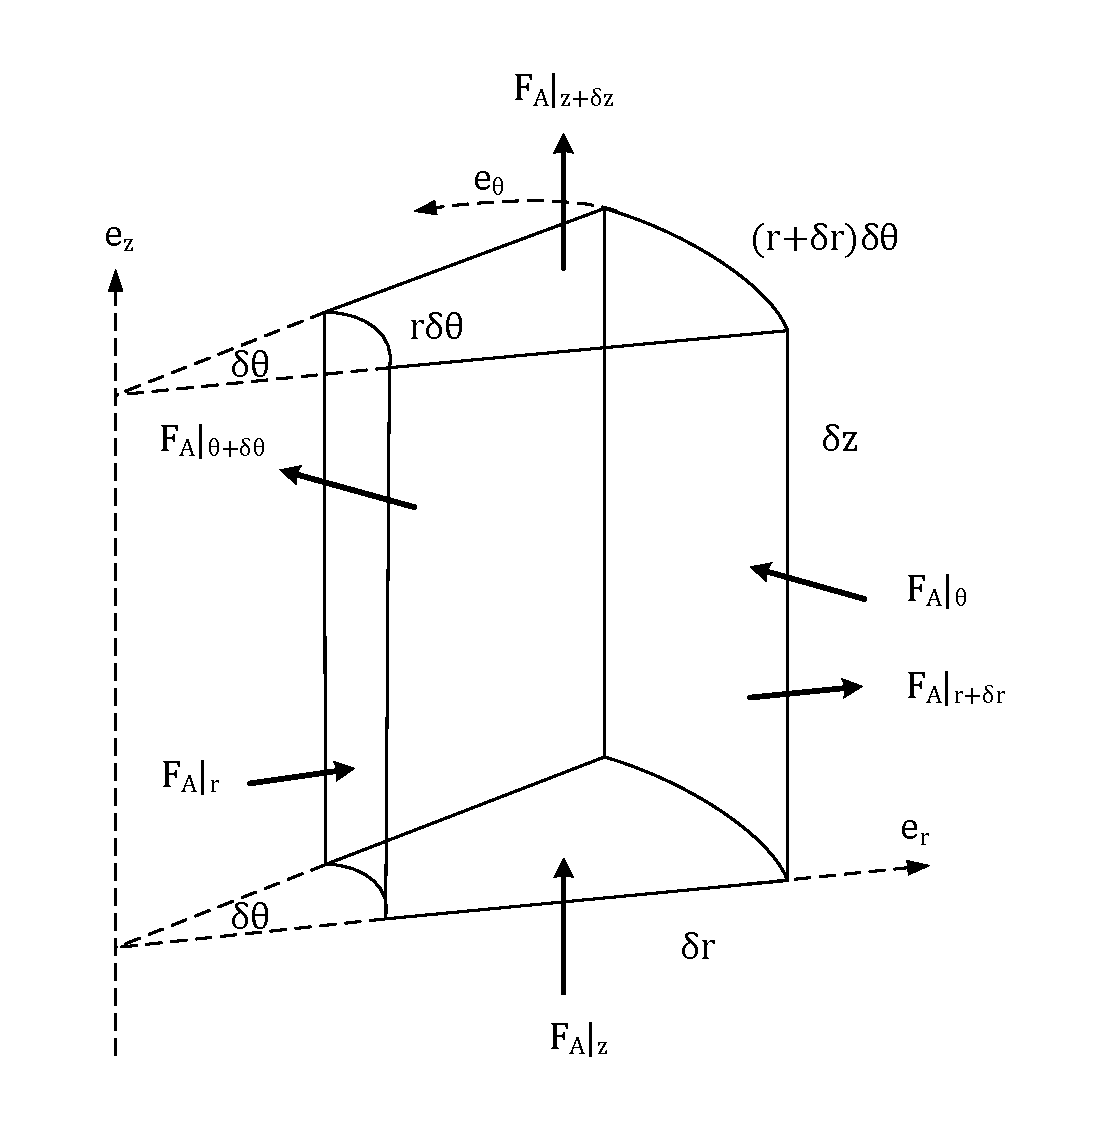
\includegraphics[scale=0.5]{volume_element}
\caption{Control volume element for a tubular reactor} 
\label{fig_vol_element}
\end{figure}

The mole balance is shown in (\ref{eq_mole_balance}) where $r_A$ indicates the generation or consumption of species A due to reaction and $C_A$ is the concentration of species A in the mixture. The term on the right hand side of (\ref{eq_mole_balance}) represents the accumulation of species A in the control volume ($\delta V$).
\begin{equation}
\sum_{i=r, \theta, z}[F_A|_i(i) - F_A|_i(i+\delta i)] + r_A \delta V = \delta V \frac{\partial C_A}{\partial t}
\label{eq_mole_balance}
\end{equation}
Consider the molar flow rate in the $\mathbf{e}_r$ direction. By using the definition of molar flux and the first order Taylor series expansion of $F_A|_r(r+\delta r)$ we have (\ref{eq_far}).
\begin{equation}
\begin{aligned}
F_A|_r(r) &= W_A|_r(r) r \delta \theta \delta z \\
F_A|_r(r+\delta r) &= (W_ A|_r(r) + \frac{\partial W_A|_r(r)}{\partial r} \delta r)(r+\delta r)\delta \theta \delta z
\end{aligned}
\label{eq_far}
\end{equation}
Neglecting higher order terms we have (\ref{eq_far2}).  
\begin{equation}
F_A|_r(r) - F_A|_r(r+\delta r)  = - (W_ A|_r(r)  + \frac{\partial W_A|_r(r)}{\partial r}r) \delta r \delta \theta \delta z
\label{eq_far2}
\end{equation}
In a similar manner, consider the molar flow rate in the $\mathbf{e}_\theta$ direction. By again using the definition of molar flux and the first order Taylor series expansion of $F_A|_\theta(\theta+\delta \theta)$ we have (\ref{eq_fat}).
\begin{equation}
\begin{aligned}
F_A|_\theta(\theta) &= W_A|_\theta(\theta) \delta r \delta z \\
F_A|_\theta(\theta + \delta \theta) &= W_A|_\theta(\theta) \delta r \delta z + \frac{\partial W_A|_\theta(\theta)}{r \partial \theta}\delta \theta\delta r \delta z
\end{aligned}
\label{eq_fat}
\end{equation}
Consequently we have (\ref{eq_fat2}).
\begin{equation}
F_A|_\theta(\theta) - F_A|_\theta(\theta + \delta \theta) =- \frac{\partial W_A|_\theta(\theta)}{r \partial \theta}\delta \theta\delta r \delta z
\label{eq_fat2} 
\end{equation}
Finally, consider the molar flow rate in the $\mathbf{e}_z$ direction. By using the definition of molar flux, the first order Taylor series expansion of $F_A|_z(z+\delta z)$, approximating the cross-sectional area normal to $\mathbf{e}_z$ in Figure \ref{fig_vol_element} as a trapezium and neglecting higher order terms, we have (\ref{eq_faz}).
\begin{equation}
\begin{aligned}
F_A|_z(z) &= W_A|_z(z) r \delta r \delta \theta \\
F_A|_z(z + \delta z) &= W_A|_z(z) r \delta r \delta \theta + \frac{\partial W_A|_z(z)}{\partial z}r \delta z \delta r \delta \theta
\end{aligned}
\label{eq_faz}
\end{equation}
Consequently we have (\ref{eq_faz2}).
\begin{equation}
F_A|_z(z) - F_A|_z(z + \delta z) = - \frac{\partial W_A|_z(z)}{\partial z}r \delta z \delta r \delta \theta
\label{eq_faz2}
\end{equation}
Substituting (\ref{eq_far2}), (\ref{eq_fat2}) and (\ref{eq_faz2}) into (\ref{eq_mole_balance}) results in (\ref{eq_mb2}). Note that for sufficiently small $\delta r$ we have $\delta V \approx r \delta \theta \delta r \delta z$.
\begin{equation}
- (W_ A|_r(r)  + \frac{\partial W_A|_r(r)}{\partial r}r) \delta r \delta \theta \delta z - \frac{\partial W_A|_\theta(\theta)}{r \partial \theta}\delta \theta\delta r \delta z - \frac{\partial W_A|_z(z)}{\partial z}r \delta z \delta r \delta \theta + r_A \delta V = \delta V \frac{\partial C_A}{\partial t}
\label{eq_mb2}
\end{equation}
Dividing through by $r \delta \theta \delta r \delta z$ results in (\ref{eq_mb3}) which is equivalent to (\ref{eq_mb4}).
\begin{equation}
-\frac{1}{r} W_A|_r - \frac{\partial W_A|_r}{\partial r} - \frac{1}{r^2}\frac{\partial W_A|_\theta}{\partial \theta} - \frac{\partial W_A|_z}{\partial z}+ r_A  = \frac{\partial C_A}{\partial t}
\label{eq_mb3}
\end{equation}
\begin{equation}
-\frac{1}{r} \frac{\partial (rW_A|_r)}{\partial r} - \frac{1}{r^2}\frac{\partial W_A|_\theta}{\partial \theta} - \frac{\partial W_A|_z}{\partial z}+ r_A  = \frac{\partial C_A}{\partial t}
\label{eq_mb4}
\end{equation}
It is now necessary to make modelling assumptions. Firstly, we will neglect any variations in the rotational direction (modelled by assuming $\frac{\partial W_A|_\theta}{\partial \theta} \approx 0$).

Secondly, we assume that Fick's Law is valid, that the diffusivity ($D_{AB}$) is constant and that the total concentration of the system is constant. This last assumption limits us to considering only reactions which conserve the total number of moles e.g. $A \rightarrow B$ or $A + B \rightarrow 2C$ etc..

Thirdly, we assume that the convection in the radial direction is negligible and that the velocity profile of molar flow in the axial direction only varies in the radial direction ($U(z,r)=U(r)$). These assumptions are not particularly strong but nevertheless simplify the model considerably. The resultant constitutive equations are shown in (\ref{eq_fick}).  
\begin{equation}
\begin{aligned}
W_A|_z &= -D_{AB}\frac{\partial C_A}{\partial z} + C_A U(r) \\
W_A|_r &= -D_{AB}\frac{\partial C_A}{\partial r}  
\end{aligned}
\label{eq_fick}
\end{equation} 
Substituting (\ref{eq_fick}) into (\ref{eq_mb3}) results in the model (\ref{eq_cdr}) we will be using for this project \cite{fogler}.
\begin{equation}
D_{AB}(\frac{1}{r}\frac{\partial}{\partial r}(r\frac{\partial C_A}{\partial r}) + \frac{\partial^2 C_A}{\partial z^2}) - U_z\frac{\partial C_A}{\partial z} + r_A = \frac{\partial C_A}{\partial t}
\label{eq_cdr}
\end{equation}
Up to now not much has been said about the reaction term $r_A$. Typically $r_A$ is formulated as a rate equation based on experimental evidence modelling reaction kinetics. It is possible for the rate ``law" to be quite complex in character but the most commonly encountered expressions for forward, irreversible reactions are based on power law kinetics \cite{delmar}. For example, it usually takes the form $-r_A=k(T)[C_A]^M$ for reactions of the form $A \rightarrow B$ or $-r_A=k(T)[C_A]^M[C_B]^N$ for reactions of the form $A + B \rightarrow 2C$ with $M,N$ usually a non-negative integer less than 3. The factor $k(T)$ is called the rate constant even though it is not a constant (it depends quite strongly on temperature). The Arrhenius equation is a very commonly used empirical function which describes the temperature dependence of the rate constant. It is typically expressed by (\ref{eq_arrhenius}) with $E$ is the activation energy, $R$ the ideal gas constant and $k_a$ is the pre-exponential factor at the reference temperature $T_a$. 
\begin{equation}
k(T) = k_a e^{(\frac{E}{R}(\frac{1}{T_a} - \frac{1}{T}))}
\label{eq_arrhenius}
\end{equation} 
It is prudent (in practice a necessity) to attempt to model the temperature profile of the reactor. We start the derivation by considering the first law of thermodynamics for an open system again applied to the control volume in Figure \ref{fig_vol_element}. In (\ref{eq_ftd}) $F_{i0}$ and $F_{i}$ denotes the molar flow of species $i$ into and out of the control volume respectively, and similarly with the energy $E$. The law states that the rate of change of energy in a system is the sum of the heat flow ($\dot{Q}$) to the system minus the work done ($\dot{W}$) by the system plus the rate of energy transferred due to flow (the last two terms). 
\begin{equation}
\frac{d E_{syst}}{dt} = \dot{Q} - \dot{W} + \sum F_{i0}E_{i0} -\sum F_{i}E_{i}
\label{eq_ftd}
\end{equation}
\begin{rmrk}
More precisely the flow terms should be vector valued due to the choice of the control volume. This is suppressed at the moment for the sake of clarity. Additionally, unless otherwise stated, $\sum$ is actually the sum over all species in the control volume i.e. $\sum_{i=1}^{N}$ where $i=1$ would indicate species 1 etc. 
\end{rmrk}
It is customary to separate the work term into shaft and flow work terms as in (\ref{eq_work}). In this equation $\hat{V}_i$ indicates the specific molar volume of species $i$.
\begin{equation}
\dot{W} = -\sum F_{i0}P\hat{V}_{i0} + \sum F_{i}P\hat{V}_{i} + \dot{W}_s
\label{eq_work} 
\end{equation}
Substituting this into (\ref{eq_ftd}) we have (\ref{eq_ftd2}).
\begin{equation}
\frac{d E_{syst}}{dt} = \dot{Q} - \dot{W}_s + \sum F_{i0}(E_{i0}+P\hat{V}_{i0}) -\sum F_{i}(E_{i}+P\hat{V}_{i})
\label{eq_ftd2}
\end{equation}
Now by assuming that the energy $E_i$ is approximately equal to the internal energy $U_i$ (this assumption implies that the potential energy, kinetic energy etc. of the system is dwarfed by the internal energy), and by making use of the definition of enthalpy, $H_i = U_i + P\hat{V}_i$, we can simplify (\ref{eq_ftd2}) to (\ref{eq_ftd3}).
\begin{equation}
\frac{d E_{syst}}{dt} = \dot{Q} - \dot{W}_s + \sum F_{i0}H_{i0} -\sum F_{i}H_{i}
\label{eq_ftd3}
\end{equation} 
Now consider the left hand side of \ref{eq_ftd3}. By definition $E_{syst} = \sum N_iE_i$ where $N_i$ is the number of moles of species $i$ in the system. By using the definition of concentration ($C_i = \frac{N_i}{\delta V}$) and noting that due to our earlier assumptions $E_i = H_i - P\hat{V}_i$  we have (\ref{eq_syse}).
\begin{equation}
\frac{d E_{syst}}{dt} = \delta V \frac{\partial}{\partial t}(\sum C_i (H_i - P\hat{V}_i))
\label{eq_syse}
\end{equation}
Expanding the right hand side of (\ref{eq_syse}), assuming constant pressure and making use of the definitions of the specific molar volume ($\sum \hat{V}_iC_i = 1$) and enthalpy at constant pressure ($dH_i = C_{p_i}dT$) we have (\ref{eq_syse2}).
\begin{equation}
\frac{d E_{syst}}{dt} = \delta V \sum C_i C_{p_i} \frac{\partial T}{\partial t} + \delta V \sum H_i \frac{\partial C_i}{\partial t} 
\label{eq_syse2}
\end{equation}
If we neglect shaft work we have the general form of the first law of thermodynamics we will be using in (\ref{eq_gfl}).  
\begin{equation}
\frac{\dot{Q}}{\delta V} + \frac{1}{\delta V}\sum F_{i0}H_{i0} -\sum F_{i}H_{i} =\sum C_i C_{p_i} \frac{\partial T}{\partial t} + \sum H_i \frac{\partial C_i}{\partial t}
\label{eq_gfl}
\end{equation}
\begin{rmrk}
It now becomes necessary to consider the components of volume element  in Figure \ref{fig_vol_element} to take the derivation further.
\end{rmrk}
\begin{rmrk}
Since we neglected rotational variance in the final form of the CDR equation we will immediately neglect the angular component of the volume element in the following analysis.  
\end{rmrk}
Consider energy flow terms $\frac{1}{\delta V}\sum F_{i0}H_{i0} -\sum F_{i}H_{i}$ from (\ref{eq_gfl}) in the $\mathbf{e}_r$ and $\mathbf{e}_z$ directions for a particular species A. Using the same analysis as with the CDR derivation we have (\ref{eq_tcp1}).
\begin{equation}
\begin{aligned}
F_{A0}|_r H_{A0}(r) - F_{A}|_rH_{A}(r+\delta r) &= -(W_A|_r H_A(r) + \frac{\partial W_A|_r H_A(r)}{\partial r}r)\delta r \delta \theta \delta z \\
F_{A0}|_z H_{A0}(z) - F_{A}|_z H_{A}(z+\delta z) &= -\frac{\partial W_A|_z H_A(z)}{\partial z}r \delta r \delta \theta \delta z   
\end{aligned}
\label{eq_tcp1}
\end{equation}
Summing over all the components in the control volume and noticing that this resembles the flux terms in (\ref{eq_mb3}) we can rewrite (\ref{eq_gfl}) into (\ref{eq_tcp2}).
\begin{equation}
\frac{\dot{Q}}{\delta V} - \frac{1}{r}\frac{\partial}{\partial r}(r\sum W_i|_r H_i) - \frac{\partial}{\partial z}(\sum W_i|_z H_i) =\sum C_i C_{p_i} \frac{\partial T}{\partial t} + \sum H_i \frac{\partial C_i}{\partial t}
\label{eq_tcp2}
\end{equation}
Assuming that we can neglect the change in enthalpy in the radial direction and expanding the derivatives we have (\ref{eq_tcp3}).
\begin{equation}
\frac{\dot{Q}}{\delta V} - \sum H_i (\frac{1}{r}\frac{\partial}{\partial r}(r W_i|_r)+\frac{\partial}{\partial z}(W_i|_z)) - \sum W_i|_z \frac{\partial H_i}{\partial z} =\sum C_i C_{p_i} \frac{\partial T}{\partial t} + \sum H_i \frac{\partial C_i}{\partial t}
\label{eq_tcp3}
\end{equation}
Now note that we can substitute in (\ref{eq_mb4}) (without the rotational term) to get to (\ref{eq_tcp4}).
\begin{equation}
\frac{\dot{Q}}{\delta V} - \sum H_i r_i - \sum W_i|_z \frac{\partial H_i}{\partial z} =\sum C_i C_{p_i} \frac{\partial T}{\partial t}
\label{eq_tcp4}
\end{equation}
Now note that $\sum H_i r_i = -H_{rxn}$ where $H_{rxn}$ is the heat of reaction which we assume constant in this project (physically it is the heat added by the reaction to the system per mole reacted). We also assume that $W_i|_z \approx U_z C_i$ which is equivalent to assuming that the convective component of the axial flux dominates the diffusional component. With these assumptions we have (\ref{eq_tcp5}).
\begin{equation}
\frac{\dot{Q}}{\delta V} + H_{rxn} - U_z\sum C_{p_i}C_i \frac{\partial T}{\partial z} =\sum C_i C_{p_i} \frac{\partial T}{\partial t}
\label{eq_tcp5}
\end{equation}




%References
\newpage
\bibliographystyle{plain}
\bibliography{research}

\end{document}